\section{Results}
\begin{figure}
  \centering%
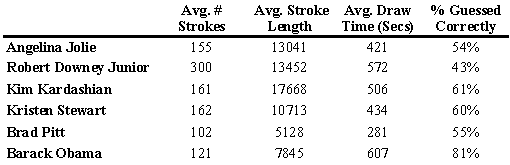
\includegraphics[height=1.1in]{./figures/daf-stats-cropped.pdf}
  \caption{Celebrity drawing statistics for 611 hand-picked drawings from the first four days after launch.}
  \label{fig:daf-stats}
\end{figure}


\begin{figure}[!t]
  \centering%
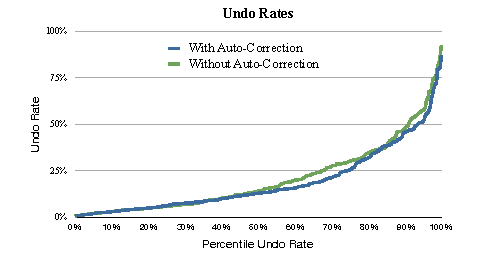
\includegraphics[width=3.5in]{./figures/userstudy/undoRates_chart_cropped.pdf}
  \caption{This chart plots the undo rates (percentage of all strokes that are undone, i.e., undos / undos+not-undos) for
each drawing sorted by undo rates. The X axis indicates the percentile undo rate, for example at the 50\% mark half of the
drawings had less undos and half more. As can be seen the two sets behave similarly for the first half in which the undo
rate is below about 15\%. However for higher percentiles the two sets diverge, with the auto-corrected drawings generally
showing lower undo rates.}
  \label{fig:daf-undos}
\end{figure}



After smaller-scale trials, \emph{DrawAFriend} was released publicly on January 8th, 2013. In 88 days there were 14,270 drawings. After the launch of \emph{DrawAFriend}, our project proceeded in three phases. First we collected drawings for six celebrities to prime our initial correction vector field. Second we use the correction field to add an automatic stroke correction helper into the game. Lastly we crowd sourced the evaluation of our stroke corrector, by AB testing it within the game.

\subsection{DrawAFriend Correction Vector Field}
In order to integrate the correction vector field into the game, we needed to prime it with some initial drawings. In four days players had downloaded the game over 2000 times and created 6373 drawings. In that time, players had already spent approximately 10 full 24 hour days drawing. We used these drawings to create the correction vector field.


Players were given the option of drawing Facebook friends or one of an initial set of six celebrities: Robert Downey Jr. \footnote{Meritano, E. "Robert Downey Jr.." Photo. wikimedia.org. Apr 2008.}, Angelina Jolie \footnote{Natt, C. "Angelina Jolie." Photo. wikimedia.org. Jun 2007.}, Kim Kardashian \footnote{Shankbone, D. "Kim Kardashian." Photo. wikimedia.org. May 2005.}, Barack Obama \footnote{Souza,P. "Barack Obama." Photo. wikimedia.org. Jan 2009.}, Brad Pitt \footnote{Boyd, B. "Brad Pitt." Photo. wikimedia.org. Mar 2008.}, or Kristen Stewart \footnote{Dispara, Atenta. "Kristen Stewart." Photo. wikimedia.org. Oct 2008.}. From the drawings generated in the first four days, we manually chose 611 celebrity drawings. In these drawings, players had made an attempt to accurately draw the eyes (the most intricate feature to draw). These 611 drawings were slightly less than 10\% of the dataset. The rest of the dataset mostly consisted of drawings that players had drawn quickly, resembling a person like scribble. While the rest of the dataset could be used for analysis, we did not train our correction vector field on it.  Figure \ref{fig:daf-stats} references statistics for these 611 drawings.

\begin{figure}[!t]
  \centering%
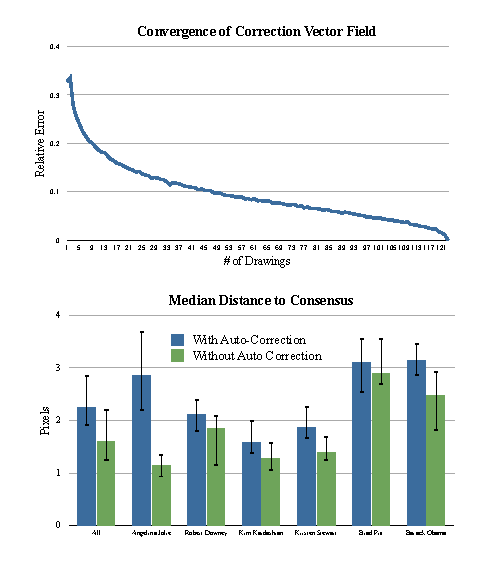
\includegraphics[width=3.5in]{./figures/userstudy/twoGraph.pdf}
  \caption{(top) Convergence of the correction vector field as more images are added. Relative error is measured between
the correction vector field built using X drawings and the correction vector field using all 124 drawings. (bottom)The
median across drawings of the mean distance of stroke points to the consensus for each celebrity with and without auto-
correction. Distance is measured by the value of the correction vector field under the strokes. The error bars mark the
60th and 40th percentile for each celebrity. Auto-correction universally leads to a greater distance, implying that users
can be sloppier when auto-correction is activated.}
  \label{fig:daf-two}
\end{figure}



We ran our modified mean shift algorithm on this initial dataset to create the correction vector fields shown in Figure \ref{fig:image-table}. Our MATLAB implementation took under 5 minutes for each celebrity.  The great majority of the time was spent in un-optimized nearest neighbor search. The dimensions of the correction vector field are 460x320. In Figure \ref{fig:daf-two} (top) we plot how our correction vector field converges for Brad Pitt. We do this by calculating the relative error between the vector field for a subset of the drawings and the vector field for all 124 drawings. There appears to be an inflection point around 25 drawings, where the the correction vector field would probably work well. However every additional drawing still improves the correction field, implying that after 124 drawings it has not completely converged. We can also use the correction vector field to filter our drawings. Drawings whose points were on average 10 pixels away from the consensus were never actually portraits (most often they were the celebrity's name spelt out). For the user study described below we used this filtering method to exclude non-portraits. 


\subsection {Drawing Enhancements}

We apply the correction vector field to interactively modify strokes during the drawing process. For every new stroke point added, a background thread is spun off to correct the new stroke. Once the thread completes if newer points have accumulated another thread is immediately spun off. Without adding user interface elements to the existing \daf UI, we seamlessly integrate stroke auto-correction. As the user draws, strokes are subtly corrected at interactive rates on an iPhone 4. In general, the fact that corrections are being applied is almost invisible to the user. Instead, strokes appear where the user {\em intended} to draw.

%????Please see the \alex{Not sure how to reference the teaser on top} and the video for interactive examples.

We also applied the correction vector field retrospectively to improve the existing database of user drawings. The drawings are already quite good, making the vector field corrections all the more impressive.  While the algorithm improves the images, it does so without sacrificing style. For comparisons of the raw drawings and the corrected images please see Figure~\ref{fig:results}, our video, and the supplementary files.

\subsection {Crowdsourced User Study}

One key advantage of developing \daf as an online game, is the ability to quickly deploy a study of users at scale. To test the effectiveness of the stroke auto-correction, we instrumented the game to enable a simple AB study. Every time a user started a drawing they were unknowingly placed in one of two groups. One group drew the celebrities as before. The other group, unbeknownst to them, drew with the stroke auto-correction on. By comparing these two groups, we can assess the effectiveness of the stroke auto-correction helper. Users drew one of the six celebrities. We use the consensus vector field to filter out drawings that could not be portraits. We record the geometry and timing of each stroke, all {\em undo}s, and the recognition rates of the players receiving the drawings.

% By adding only a couple of lines of code, we transformed a data collection crowd sourcing system into a large-scale user study.


\subsubsection {User Study Results}

After approximately one week, 500 players had "contributed" to the study to test the effect of the auto-correction on over 1300 drawings. Using this data we assess recognition rates (measuring how good drawings are from the perspective of others). We also analyze undo rates (providing an insight into how artists like their own drawings). Finally we measure average "distance" from the artistic consensus (measuring how carefully artists are drawing).

%Our results show that autocorrect reduced undo rates (the ratio of undos to all other strokes). This effect is magnified for careful drawers (who undid 30\% or more strokes). Their undo rates decreased by a significant 5\% (Wilcoxian p-value = .045).  Before we analyzed the undo rates we removed all drawings that had 0 undos (assuming most of these players did not know undo existed) and all drawings with less than 10 strokes (assuming these drawings were not actual attempts to draw the celebrity).  Figure \ref{fig:daf-three} middle shows the effect that auto correction has on decorating undo rates, particularly for more careful drawers. We view the drop in undo rates as an improvement in how players view their own drawings.

%[Someone Please Review this Paragraph]

First we investigate {\em undos} as an indication of how artists like their own drawing. Since players use different number
of strokes, we focus on undo rates, which is the number of strokes undone over the total number of strokes. For example if
a user drew 100 strokes and pressed undo for 40 of them, this would have an undo rate of 40\%. For our analysis we removed
all drawings that had 0 undos (assuming this implied players did not know undo existed). This left 327 drawings auto-corrected
 and 295 that were not. We sorted each set of drawings by the undo rates from lowest to highest, and in Figure
\ref{fig:daf-undos}, plotted the undo rate for each percentile of sorted drawings (this normalizes for the different
number of drawings in each set). The distribution of undo rates for drawings with fewer undos track together for both
sets with and without autocorrection. However the undo rates diverge further along the sorted lists. This seems to imply
that our auto-corrector lowers the undo rate for more careful drawers (players that undo a larger percent of their
strokes).

 
With auto-correct on,  we observe a significant increase in the average distance between the actual uncorrected strokes
and the consensus drawings (as measured by the \emph{correction vector field}). We perform a two-sample Wilcoxon test of
whether or not there is a difference in the mean of the correction vector field under the stroke points with auto correct
on versus off. This shows a significant difference in the means, with a p-value of $1.653*10^{-6}$.  This suggests that
artists do not need to draw as precisely. Figure \ref{fig:daf-two} (bottom) shows the median distance to the consensus for
each celebrity with a sample size of 570 auto-corrected and 533 not auto-corrected.
 

Interestingly, statistical analysis reveals that the auto-corrector does not significantly alter recognizability.
Corrected drawings had a recognition rate of $37.5\% \pm 2.02\%$ while uncorrected drawings had an average recognition
rate of $38.6\% \pm 2.11\%$ (again 570 and 533 drawings respectively). We believe that our auto-corrector does not change
players final drawing quality. Rather it makes reaching this level of quality easier by requiring less undos and less
accuracy.

\begin{figure*}[!t]
  \centering%
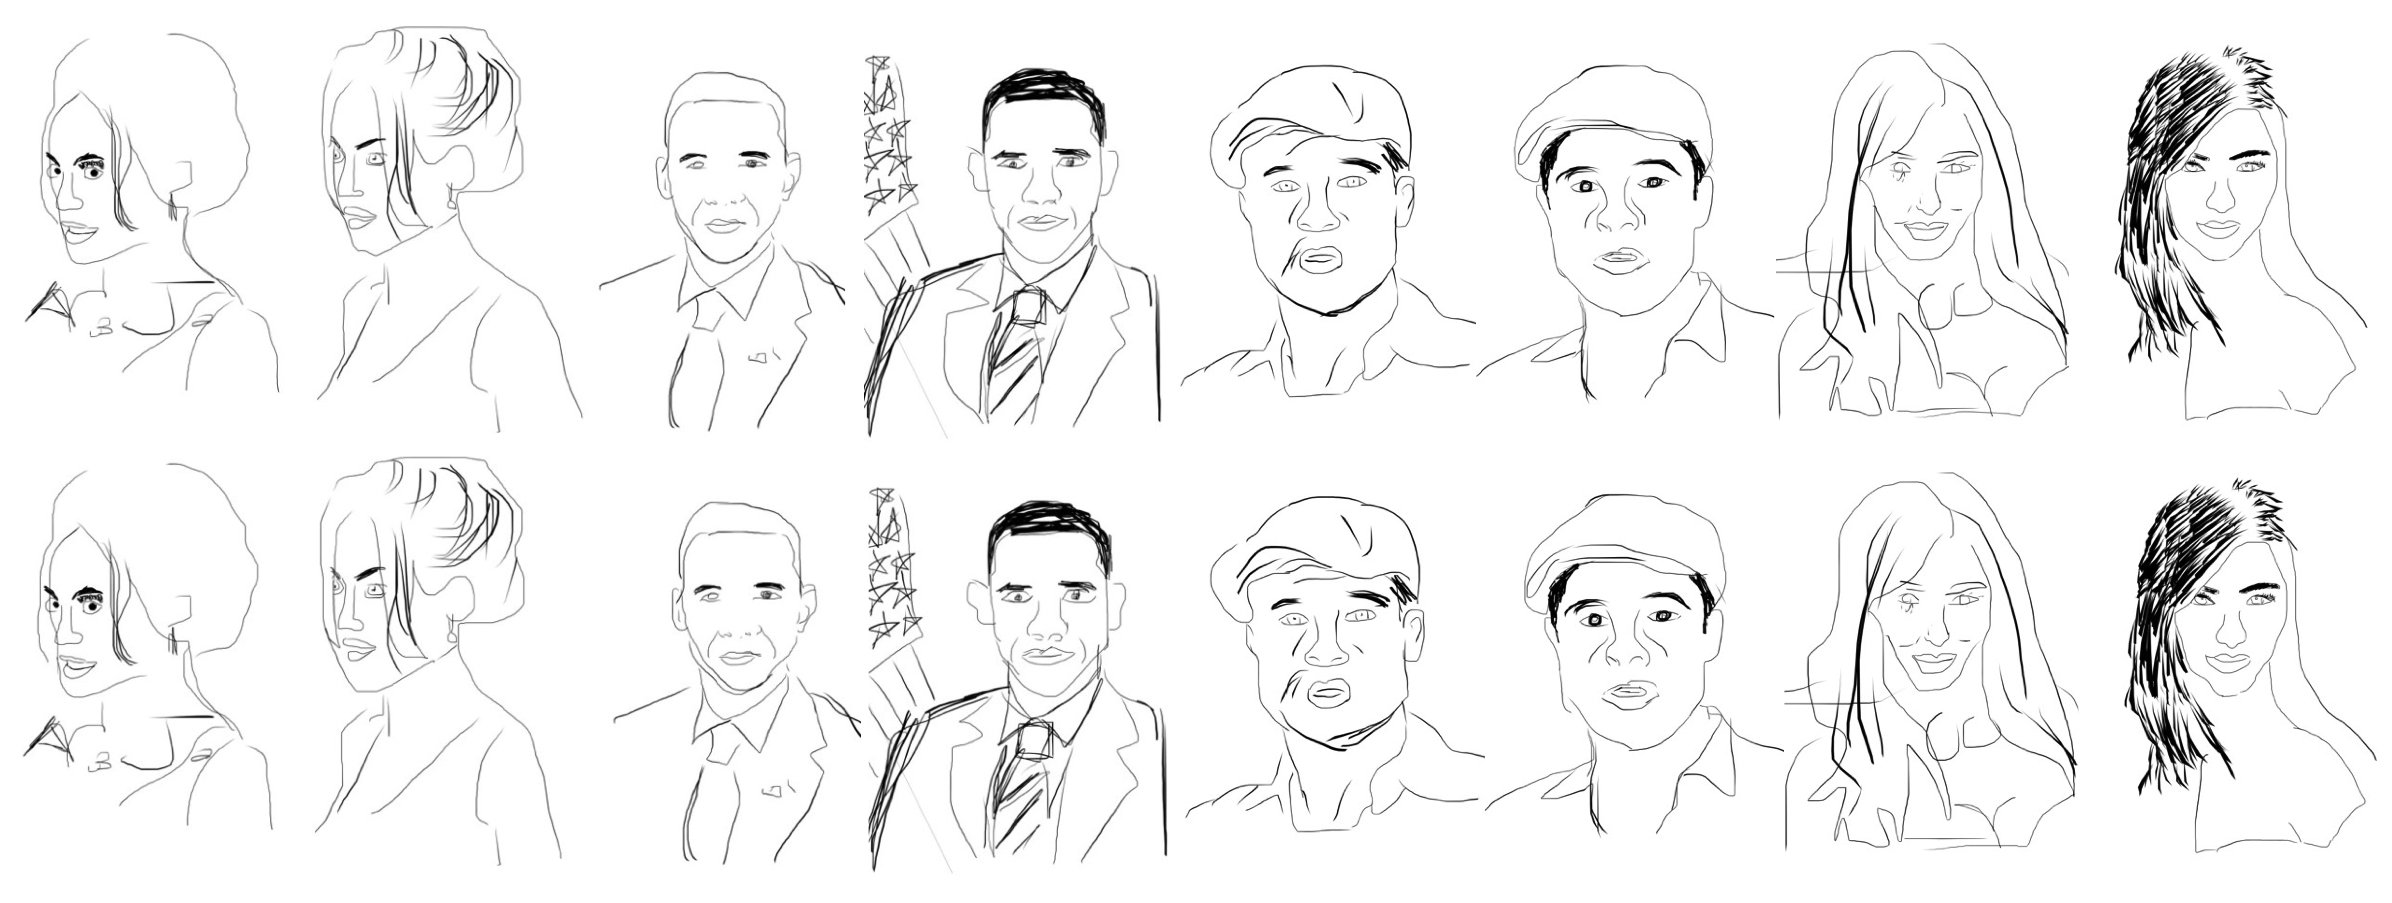
\includegraphics[width=7in]{./figures/ResultsAll_16.pdf}
\vspace{-0.35in}
  \caption{Celebrity drawings: original strokes (bottom rows) and after automatic adjustment to consensus (top rows). (Please see the supplementary files for more examples and also for an interface so you can flip between them.)}
\vspace{-0.25in}
  \label{fig:results}
\end{figure*}
